\documentclass[runningheads,a4paper,draft]{svjour3}

%\usepackage{etex}
%packages indispensables
\usepackage[utf8]{inputenc}
\usepackage{lmodern}
\usepackage{todonotes}
\newcommand{\todoi}[1]{\todo[inline]{#1}}

%\usepackage{graphicx}
%packages utiles
\usepackage{alltt} %program code
%\usepackage{enumerate}
%\usepackage{amssymb} %lettres mathématiques
%\let\oldemptyset\emptyset
%let\emptyset\varnothing
%\usepackage{amsthm}
\usepackage{amsfonts}
%\usepackage{bussproofs} %derivation 
%\usepackage{hyperref} %to write path.
%\usepackage{color} % colouring text
%\usepackage{tabularx} % table
%\usepackage{fancyvrb}
%\usepackage[toc,page]{appendix}
%\usepackage{cite}
\usepackage{booktabs}

\usepackage{tikz}
\usetikzlibrary{shapes,arrows}
\usepackage{pgfplots}
%\usepackage{float}
%\restylefloat{table}
\usepackage{xcolor}
\usepackage{url}
\usepackage{subfigure}

\usepackage{xspace}
\usepackage{amsmath}
\DeclareMathOperator*{\argmin}{\arg\!\max}
\DeclareMathOperator*{\argmax}{\arg\!\max}
\DeclareMathOperator*{\average}{Average}

\def\holfour{\textsf{HOL4}\xspace}
\def\isabelle{\textsf{Isabelle}\xspace}
\def\hollight{\textsf{HOL Light}\xspace}
\def\mizar{\textsf{Mizar}\xspace}
\def\coq{\textsf{Coq}\xspace}
\def\ocaml{\textsf{OCaml}\xspace}
\def\vampire{\textsf{Vampire}\xspace}
\def\eprover{\textsf{E-prover}\xspace}
\def\zthree{\textsf{z3}\xspace}

\def\sml{\textsf{SML}\xspace}
\def\polyml{\textsf{Poly/ML}\xspace}
\def\holyhammer{\textsf{HOL(y)Hammer}\xspace}
\def\sledgehammer{\textsf{Sledgehammer}\xspace}
\def\mizAR{\textsf{MizAR}\xspace}

\def\metis{\textsf{Metis}\xspace}
\def\leancop{\textsf{leanCoP}\xspace}
\def\tactictoe{\textsf{TacticToe}\xspace}
\newcommand{\bq}[1]{\textbackslash"{#1}\textbackslash"}
\newcommand{\ra}[1]{\renewcommand{\arraystretch}{#1}}
%\theoremstyle{remark}
%\newtheorem{example}{Example} 
%\newtheorem{remark}{Remark} 
%\newtheorem{definition}{Definition} 
\clubpenalty=10000
\widowpenalty=10000 

\usepackage{fancyvrb}
\usepackage{tikz} % graphics
% graphs
\usetikzlibrary{arrows,shapes}
\usetikzlibrary{trees,positioning,fit}
\tikzstyle{block} = [rectangle, draw,% fill=blue!20,
    text width=5em, text centered, rounded corners, minimum height=4em]
\tikzstyle{line}=[draw]
\tikzstyle{cloud} = [draw, ellipse,%fill=red!20,
    node distance=3cm,
    minimum height=2em]


% graphs
\usetikzlibrary{arrows,shapes,calc}
\usetikzlibrary{trees,positioning,fit}
\tikzstyle{arrow}=[draw,-to,thick]
\tikzstyle{bluearrow}=[draw,-to,thick,blue]
\tikzstyle{tcircle} = [circle, draw, fill=white]
\tikzstyle{tsquare} = [rectangle, draw, fill=white]
\tikzstyle{bcircle} = [circle, draw, blue, fill=blue]
\tikzstyle{gcircle} = [circle, draw, mygreen, fill=mygreen]

%\title{TacticToe: A theorem prover trained from formal proofs}
%\title{TacticToe: Smart guidance in tactical proof search}
%\title{TacticToe: Proof  by Tactic Selection}
\title{TacticToe: Learning the Game of Tactics}
%\title{TacticToe: Learning the Tactic Game}
%\title{TacticToe: Automatic tactic-level proof generation} 

\author{\mbox{Thibault Gauthier} \and \mbox{Cezary Kaliszyk} \and \mbox{Josef 
Urban} \and \mbox{Ramana Kumar} \and \mbox{Michael Norrish}}

\authorrunning{Gauthier et al.}
%\titlerunning{TacticToe: Learning to Reason with HOL4 Tactics}

\institute{Thibault Gauthier and Cezary Kaliszyk \at
Department of Computer Science, University of Innsbruck,
%Technikerstr. 21a/2,
Innsbruck, Austria\\ \url{{thibault.gauthier,cezary.kaliszyk}@uibk.ac.at}
\and
Josef Urban \at Czech Technical University, Prague\\\url{josef.urban@gmail.com}
\and Ramana Kumar and Michael Norrish \at Data61}


%\institute{
%  University of Innsbruck\\
%  \email{\{thibault.gauthier,cezary.kaliszyk\}@uibk.ac.at}
%\and
%  Czech Technical University, Prague.\\
%  \email{josef.urban@gmail.com}\\
%}


\usepackage[final]{listings}
%\usepackage[scaled=.95]{couriers}
\lstdefinelanguage{SML}%
{columns=fullflexible,
  keywords={THEN,THENL,val,open,store_thm,fun,fn},%
  frame=none,
  sensitive=true,
  keywordstyle=\fontfamily{lmss}\footnotesize\selectfont,%
  basicstyle=\fontfamily{pcr}\selectfont,%
  stringstyle=\tt,
  morestring=[b]",
  literate={\ }{$\mkern6mu$}1%
   {=}{{\tt\raisebox{-.15mm}{=}}}1%
   {[}{{\tt\raisebox{-.15mm}{[}}}1%
   {]}{{\tt\raisebox{-.15mm}{]}}}1%
   {->}{{$\rightarrow$}}1%
   {==>}{{$\Rightarrow$}}1%
   {wedge}{{$\wedge$}}1%
   {>=}{{$\geq$}}1%
   {'a}{{$\alpha$}}1%
   {'b}{{$\beta$}}1%
   {ldots}{$\ldots$}1%
   {!}{$\forall$}1%
   {``}{\hspace{-.5mm}`\hspace{-1mm}`}1%
  }

\lstdefinelanguage{SMLSmall}%
{columns=fullflexible,
  keywords={THEN,THENL,val,open,store_thm,fun,fn},%
  frame=none,
  sensitive=true,
  keywordstyle=\fontfamily{lmss}\scriptsize\selectfont,%
  basicstyle=\fontfamily{pcr}\small\selectfont,%
  stringstyle=\tt,
  morestring=[b]",
  literate={\ }{$\mkern6mu$}1%
   {=}{{\tt\raisebox{-.15mm}{=}}}1%
   {[}{{\tt\raisebox{-.15mm}{[}}}1%
   {]}{{\tt\raisebox{-.15mm}{]}}}1%
   {->}{{$\rightarrow$}}1%
   {==>}{{$\Rightarrow$}}1%
   {wedge}{{$\wedge$}}1%
   {<=}{{$\leq$}}1%
   {>=}{{$\geq$}}1%
   {'a}{{$\alpha$}}1%
   {'b}{{$\beta$}}1%
   {ldots}{$\ldots$}1%
   {!}{$\forall$}1%
   {``}{\hspace{-.5mm}`\hspace{-1mm}`}1%
  }
\lstset{language=SML}
\begin{document}
\maketitle

\todo{JU review: Still feels more like an intro than an abstract. Could be 
shorter and punchier.}
\begin{abstract}
Formalization of mathematics in interactive theorem provers (ITPs) 
relies today on many proof automation methods.
Some of these methods are general-purpose and with enough time they can prove any 
theorem. Many formalized proof scripts however also
take advantage of specialized rules and theory-based strategies. 
In the HOL4 ITP system, practically all of them are implemented as \emph{tactics}. 

Automated theorem provers (ATPs) rely on parameterizable general 
strategies. Sometimes, a strategy can be specialized for only one theory as in 
SMT solving. But it is difficult for an automated theorem prover to rely on 
rules tailored for a particular case. 
Indeed, this would require implementing many specific rules and more 
importantly figuring out in which cases they can be applied. 

We bridge this gap by implementing our tactical prover TacticToe on top 
of the HOL4 ITP. 
TacticToe first learns from many proof scripts
the relevance of tactics in particular proof situations.
This learned knowledge is then used in a Monte Carlo tree search algorithm that explores the most promising tactic-level proof paths. 
On a single CPU, with a time limit of 60 seconds, TacticToe proves 66.2\% 
of 7164 theorems of the standard library where as 
Eprover solves 34.5\%. The success rate rises to 69.0\% by combining the 
result of both provers.
\end{abstract}

\section{Introduction}
\tableofcontents

\todo{Comparison with hammers in usability}
Many of the state-of-the-art interactive theorem provers (ITPs) such as
  \holfour~\cite{hol4}, \hollight~\cite{Harrison09hollight}, 
  \isabelle~\cite{isabelle} 
  and \coq~\cite{coq-book}
  provide high-level parameterizable tactics for constructing the
  proofs.  Such tactics typically analyze the current goal state and
  assumptions, apply nontrivial proof transformations, which get
  expanded into possibly many basic kernel-level inferences or significant 
  parts of the proof term.
%\marginpar{not Coq}
  In this
  work we develop a tactic-level automation procedure for the \holfour ITP
  which guides selection of the tactics by learning from previous
  proofs.  Instead of relying on translation to first-order automated
  theorem provers (ATPs) as done by the hammer 
  systems~\cite{hammers4qed,tgck-cpp15}, the technique
%\marginpar{too many cites?}
%BlanchetteGKKU16,holyhammer,mizAR40
  directly searches for sequences of tactic applications that lead to
  the ITP proof, thus avoiding the translation and
  proof-reconstruction phases needed by the hammers.

\todo{Rewrite the plan}
  To do this, we \emph{extract and record} tactic invocations from the ITP 
  proofs (Section~\ref{sec:recording}) and
  \emph{build efficient machine learning classifiers} based on such training
  examples (Section~\ref{s:prediction}).  The learned data serves as a 
  guidance for a \emph{Monte Carlo tree search} that explores the different 
  proof paths (Section~\ref{sec:proofsearch}). The result, if
  successful, is a certified human-level proof composed of \holfour
  tactics.  The system is evaluated on a large set of theorems originating
  from \holfour (Section~\ref{s:experiments}), and we show that the performance 
  of the single best \tactictoe strategy exceeds the performance of a hammer 
  system used with a single strategy and a single efficient external prover.


\subsection{The problem}
How a user works with an ITP and how this gives rise to a machine learning 
problem.
Two ways of representing a formulas.
Definition of a tactic in \holfour. In this research, we will take the definition
that a tactic takes a goal and returns a list of goals.
Input of the prediction: goal
If a tactic produces no goals then its input goal is solved.




\subsection{Contributions}
This work is an extension of the work described in \cite{tgckju-lpar17}.
There we proposed the idea of ... and achieved ...
The additional contributions and their effect on our system are:

\todoi{add prediction of 3 kinds of things}
\begin{itemize}
\item Proof recording at the tactic level is made more precise. Pattern 
matching constructions, opening of submodules are supported. The different 
recording steps (parsing, unfolding and replaying) are regrouped into a single 
\sml function. So, our recording is more complete and fully automatized.
\item Two types of arguments (list of theorems and terms) can be predicted 
independently of the tactic. Combinatorial explosion in the number of tactics 
is prevented through the introduction of abstracted tactics. As desired, their 
instantiations is dependent on the target goal.
\item MCTS (Monte Carlo tree search) now replaces A* in our proof search 
algorithm. MCTS gives a more balanced feedback to guide proof search by 
comparing subtrees instead of leafs. The policy and evaluation are learned 
through supervised learning.

\item First evaluation of \tactictoe and \eprover success rates relative to 
the length of the original proofs.
\item User interaction is enhanced by the minimization and prettification 
applied on the generated proof.
\item The internal ATP \metis used during proof search can be complemented 
by asynchronous calls to \eprover.
\end{itemize}



\section{Preliminaries: Search Tree}\label{sec:prelim}
\todoi{Print words correctly in math format by avoiding math format}  

In order to be able to describe the different components of \tactictoe, 
we need to give to describe what a search tree is, what are its elements and 
how they are organized relative to one other. The following description is 
static and the evolution of the search tree toward a proof is given in 
Section~\ref{sec:proofsearch}.

\begin{definition}(search tree)\\
A search tree $\mathfrak{T}$ is a sixtuple 
$(\mathbb{T},\mathbb{G},\mathbb{A},T,G,A)$ 
that respects the following conditions:
\begin{itemize}
\item $\mathbb{T}$ is a set of tactics, $\mathbb{G}$ is a set of goals 
 and $\mathbb{A}$ is a set of nodes. These sets contains only objects 
 appearing in the search tree.
\item $T$ is a total function from $\mathbb{G}$ to $P(\mathbb{T})$. It takes a 
goal and return the set of tactics already applied to this goal.
\item $G$ is a total function from $\mathbb{A}$ to $P(\mathbb{G})$. It takes a 
node a return the set of goals in this node.
\item $Support(A) = \lbrace (g,t)\ |\ t \in T(g) \rbrace$.
\item $A$ is a partial function from $\mathbb{G} \times \mathbb{T}$ to 
$\mathbb{A}$. It takes a goal and a tactic and returns the node produced by the 
application of the tactic to the goal, if this tactic has been applied to this 
goal.
\item if $t \in T(g)$ and $A(g,t) = a$ then $t(g) = G(a)$.
\end{itemize}

Additional constraints such as acyclicity and the fact that there is exactly 
one root node are properties of this graph that are preserved during the 
application of the MCTS algorithm. That is why we call it a tree although this 
is not specified in this definition.
\end{definition}

If no explicit order is given, we assume that any set is equipped with an 
arbitrary order. In this way, we can access the nth member of set $s$ by 
writing $s_n$. In Figure~\ref{fig:choice}, $(G(a_j))_i$ is written $g_j^i$.

\begin{figure}{}
\begin{center}
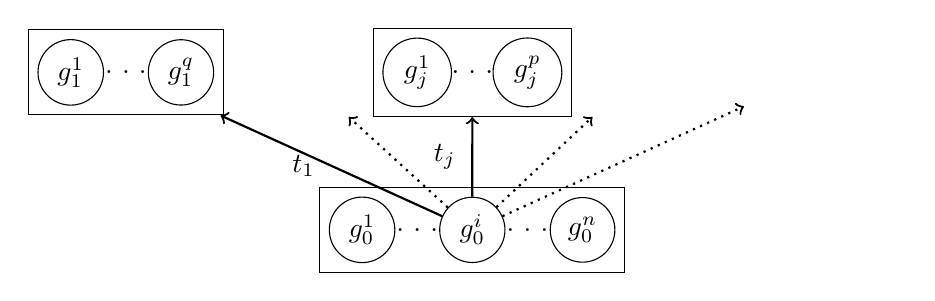
\begin{tikzpicture}[node distance=0.7cm]
\node [tcircle] (0) {$g_0^i$};
\node [right of=0] (0r) {.\ .\ .};
\node [tcircle,right of=0r] (0rr) {$g_0^n$};
\node [left of=0] (0l) {.\ .\ .};
\node [tcircle,left of=0l] (0ll) {$g_0^1$};
\node [draw,fit=(0rr) (0ll)] {}; 
\node [above of=0,node distance=2cm] (2) {.\ .\ .};
\node [left of=2, tcircle] (2l) {$g_j^1$};
\node [tcircle,right of=2] (2r) {$g_j^p$};
\node [draw, fit=(2l) (2r)] (2b) {}; 

\node [tcircle, left of=2l, node distance=3cm] (1r) {$g_1^q$};
\node [left of=1r] (1) {.\ .\ .};
\node [tcircle, left of=1] (1l) {$g_1^1$};
\node [draw, fit=(1l) (1r)] (1b) {}; 

\node [right of=2r,node distance=3cm] (3l) {$\phantom{g_3^p}$};
\node [right of=3l] (3) {\phantom{.\ .\ .}};
\node [right of=3] (3r) {$\phantom{g_3^p}$};
\node [fit=(3l) (3r)] (3b) {};

\node [fit=(1r) (2l)] (1m) {}; 
\node [fit=(2l) (3r)] (2m) {}; 

\draw[-to,thick] (0) to node[xshift=-10](t1){$t_1$} (1b);
\draw[-to,thick] (0) to node[xshift=-10](t2){$t_j$} (2b);
\draw[-to,dotted,thick] (0) to (1m);
\draw[-to,dotted,thick] (0) to (2m);
\draw[-to,dotted,thick] (0) to (3b);
\end{tikzpicture}
\end{center}
\caption{A node of a search tree and the children of one of 
its goal.}
\label{fig:choice}
\end{figure}

Starting from the bottom parent node, we can construct children of a goal of 
this node by choosing a goal $g_i^0$ on this node and choosing tactics 
$t_1,t_2,\ldots$ to 
apply to this goal. Here the result produces new nodes each containing a list 
of goals to be proven. In each node of the proof tree, a goal can either be 
solved, open or pending (see Definition~\ref{def:solved}). 

In the following, new concepts and properties are defined in the context of a 
search tree $\mathfrak{T}$.


\begin{definition}\label{def:solved}(Solved goal, solved nodes, open goal, 
pending goal)\\
The set of solved nodes $\mathbb{A}^\infty$ and 
the set of solved goals $\mathbb{G}^\infty$ are defined inductively by:

\begin{align*}
\mathbb{A}^{0} &=_{def} 
\lbrace a \in \mathbb{A}\ |\ G(a) = \emptyset \rbrace \\ 
\mathbb{G}^{0} &=_{def} \lbrace g \in \mathbb{G}\ |\ 
\exists a \in A(g).\ a \in \mathbb{A}^{0} \rbrace\\
\mathbb{A}^{n+1} &=_{def} \lbrace a \in \mathbb{A}\ |\ 
\forall g \in G(a).\ g \in \mathbb{G}^{n} \rbrace\\
\mathbb{G}^{n+1} &=_{def} \lbrace g \in \mathbb{G}\ |\ 
\exists a \in A(g).\ a \in \mathbb{A}^{n+1} \rbrace \\
\mathbb{A}^\infty &=_{def} \bigcup_{n \in \mathbb{N}} \mathbb{A}^n \ \ \ \ \ 
\mathbb{G}^\infty =_{def} \bigcup_{n \in \mathbb{N}} \mathbb{G}^n\\
\end{align*}

An open goal is an unsolved goal that was tried at least once by a tactic. The 
set of open goals can be formally defined as:  
\[\lbrace g \in G\ |\  T(g) \neq \emptyset \wedge g \notin \mathbb{G}^\infty 
\rbrace\]

The set of pending goals is the remaining set of goals in the tree. They are 
goal that were produced by tactics that were not explored yet. This set can 
also be also defined by:
\[\lbrace g \in G\ |\  T(g) = \emptyset \rbrace\]

To facilitate the description  of our algorithms we make a slight adjustement 
to the definition of an open goal. If a node $a$ does not contain any open 
goal, the first pending goal (according 
to some preset order) of $a$ is also considered to be an open goal. In this 
way, each unsolved node contains a unique open goal.
\end{definition}


We can also judge the productivity of a tactic by its contribution to the 
search 
tree. 

\begin{definition} (Productive tactic) 
The application of a tactic on an open goal is called productive if and only if 
all the following conditions are satisified:
\begin{itemize}
\item It does not fail or timeout. To prevent tactics from looping, we 
interrupt tactics after a short amount of time (0.05 seconds). 
\item It does not loop. Its output does not contain any goals that appears in 
its ancestor nodes.
\item It is not a parallel step. Its output is not equal or a superset 
of a list of goals produced from the same open goal.
\end{itemize}

The third point of the definition is a partial attempt at preventing confluent 
branches. The general case where two branches join after $n$ steps is handled 
by a tactic cache which memorizes tactic effects on goals. This
cache allows faster re-exploration of confluent branches which remain 
separated in the search tree.
\end{definition}

\begin{definition}\label{def:desc}(Children, descendant, active node)\\
We now define what are the children and the descendants of a node $a$. The 
children of a relative to a goal $g$ in $G(a)$ 
is the set of nodes produced by tactics applied to $g$:
  \[Children(a,g) = \lbrace A(g,t)\in \mathbb{A}\ |\ t \in T(g) \rbrace \]

If $g$ is the open goal of $a$, then we simply call children of a the 
children of $a$ relative to $g$. We define:\\

Extended children of $a$ by:
  \[ExtChildren(a) = \bigcup_{g \in G(a)} Children(a,g) \]

Descendants of $a$ by:
\begin{align*}
Descendant^{0}(a) &=_{def} \lbrace a \rbrace \\ 
Descendant^{n+1}(a) &=_{def} \bigcup_{a' \in Descendant^{n}(a)} 
ExtChildren(a') \\
Descendant(a) &=_{def} \bigcup_{n \in \mathbb{N}} Descendant^n(a)\\
\end{align*}

Descendants of $a$ through $g$ by:
\[Descendant(a,g) =_{def} 
  \lbrace a \rbrace \cup \bigcup_{a' \in Children(a,g)} Descendant(a')\]


An active node is by definition a node that is not a descendant of a 
solved node. Non-active nodes are not worth exploring.

\end{definition}

\section{Prediction}\label{s:prediction}
The learning-based selection of relevant lemmas significantly improves the 
automation for hammers~\cite{BlanchetteGKKU16}. In \tactictoe, we adapt 
one of the strongest lemma selection 
methods: the modified distance-weighted \emph{$k$ nearest-neighbour} 
classifier~\cite{ckju-pxtp13,DudaniS76} to predict three different objects: 
 tactics, theorems and list of goals. 

We first introduce specificities associated with the prediction of each object. 
In particular, we present the dataset from which objects are selected and the 
purpose of the selection process. 
We then explain the construction of the similarity measure by which relevant 
objects are predicted.

\paragraph{Tactics}
To start with, we build a database of tactics consisting
of tactic-goal pairs recorded from successful tactic applications in human 
proofs (see 
Section~\ref{sec:recording}).
Then, during proof search, we order recorded goals according to their 
similarity with a targeted goal $g$ (usually the first pending goal of a node). 
This induces 
through the recorded pairs an 
order on tactics. The intuition is that tactics which have been successful on 
goals similar to $g$ should be tried first, since they are more likely to lead 
to a proof. 
This predicted tactic order is translated into a prior policy for our MCTS 
algorithm (see Section~\ref{sec:policy}).
Tactic selection is also used to improve the quality of the database 
of tactics during orthogonalization (see Section~\ref{sec:ortho}).

\paragraph{Theorems as Argument of Tactics}
We first collect a set of theorems for our theorem predictor to select from.
It includes the \holfour theorem database and theorems from the local namespace.
Predicted tactics during proof search and orthogonalization may include
tactics where arguments (list of theorems) have been erased (see Section 
\ref{sec:synthesis}).
We instantiate those tactics by theorems that are syntactically the closest to 
the targeted goal as they are more likely to help.
The same algorithm selects suitable premises for ATPs integrated with  
\tactictoe (see Section~\ref{sec:atp}).

\paragraph{List of Goals as Output of Tactics}
A dataset of tactic outputs is compiled during orthogonalization (see 
Section~\ref{sec:evaluation}).
This set is separated into positive and negative examples.
List of goals that subsumes the result of an original tactic on a 
targeted goal are considered positive. During proof search, given a list of 
goals $l$ created by a tactic, we select a set of lists of goals that are most 
similar to $l$. The ratio of positive examples in the selection gives us a 
prior evaluation for MCTS.


\subsection{Feature Extraction}\label{sec:features}
The three objects considered are different representation of mathematical 
formulas. Therefore, we start by describing which features we extract can 
extract terms. From there, we extend the extraction mechanism 
to goals, theorems and lists of goals. Duplicated features are always removed 
so that each object has an associated set of features.


Here are the different kind of feature we extract from terms:
\begin{itemize}
\item names of constants, including the logical operators,
\item type constructors present in the types of constants and variables,
\item subterms with all variables replaced by a single place holder $V$.
\item names of the variables.
\end{itemize}

Since goals and theorems are represented by a couple of a list of terms 
(assumptions) and a term (conclusion). We compute their features by extracting 
the features of all terms describing them. Additionally, we distinguish between 
features of the assumptions and features of the conclusion by adding a 
different tag to elements of each set. Features of a list of goals are
the union of the features of each goal in the list. 

\subsection{Similarity}\label{sec:predictions}
We estimate the similarity (or co-distance) between two objects $o_1$ and $o_2$ 
through their respective feature sets $f_1$ and $f_2$.
%The similarity function $sim$ computed by the k-NN algorithm is analogous 
%to the one used in the premise selection task~\cite{ckju-pxtp13}.
The estimation is based on the frequency of the features in the intersection of 
$f_1$ and $f_2$. A good rule of thumb is that the rarer the shared features 
are, the more similar two goals should be. The relative rarity of each feature 
can be estimated by calculating its TF-IDF weight~\cite{Jones72astatistical}.
We additionally modify the weight by raising them to the sixth power giving 
even more credence 
to rare features which was found experimentally optimal in \cite{}.\todo{CK: 
citation}

The first co-distance $sim_1$ adds the weight of each shared 
features to compute the total score.
In a second co-distance $sim_2$, we additionally take into account 
the total number of features to reduce the seemingly unfair advantage of big 
feature sets in the first scoring function.
\[sim_1 (o_1, o_2) = {\sum\nolimits_{\,f \in f_0 \cap 
f_1}{\text{tfidf}(f)^{6}}}\]
\[sim_2 (o_1, o_2) = \frac{{\sum\nolimits_{\,f \in f_0 \cap 
f_1}{\text{tfidf}(f)^{6}}}}
{ln (e + card(f_0) + card(f_1))}\]

In our setting, making prediction for an object $o$ consists of sorting a set 
of objects by their similarity to $o$. We use $sim_1$ for tactics and theorems 
and $sim_2$ for list of goals. The reason why $sim_1$ is adapted for
predicting tactics is that tactics effective on large goal $g$ are often also  
suitable for a goal made of sub-formulas of $g$. The same monotonicity 
heuristic can justify the use of $sim_1$ in theorems. Indeed in practice, a 
large theorem is often a conjunction of theorems from the same domain. 
And if a conjunction contains a formula related to a problem, then the other 
conjuncts from the same domain may also help to solve it.

\subsection{Preselection}\label{sec:dependencies}

In order to speed up the predictions during the search for a proof of a 
conjecture $c$, we preselect 500 tactic-goal pairs and theorems. 
Preselection for list of goals is induced by the preselection of input 
goals in tactic-goal pairs. Those will be the only objects available to 
\tactictoe's search algorithm for proving $c$.

The first idea is to select tactic-goal pairs and theorems by their distance to 
the conjecture. However, this selection may not be adapted to later stages of 
the proof where goals may have derived significantly from the 
initial conjecture $c$. In order to 
anticipate the production of diverse goals, our prediction during preselection
takes into account dependencies between objects of the same dataset.
The dependence relation is assymetric. Through the relation, each object has 
multiple children and at most one parent.
Once a dependency relation is established, we can calculate a dependency score 
for each object which is the maximum of its similarity score and the similarity 
score of its parent. In the end, the 500 entries with highest dependency score 
are preselected in each dataset.

In the following, we give a mathematical definition for the dependency relation 
between labels for tactic-goal pairs and theorems.

\begin{definition}(Dependencies of a tactic-goal pair)\\
Let $\mathfrak{F}$ be the set of recorded tactic-goal pairs.
The dependencies $D_\infty$ of a tactic-goal pair $(t_0,g_0)$ is 
inductively defined by:

\begin{align*}
D_0 &=_{def} \lbrace (t_0,g_0) \rbrace \\
D_{n+1} &=_{def} D_n \cup \lbrace (t,g)\in \mathfrak{F}\  |\ \exists 
(\hat{t},\hat{g}) \in D_n.\ g \in \hat{t}(\hat{g}) \rbrace  \\
D_\infty &=_{def} \bigcup_{i \in \mathbb{N}} D_i\\
\end{align*}
where $\hat{t}(\hat{g})$ denotes the resulting set of goals produced by the 
application 
of the tactic $\hat{t}$ to the goal $\hat{g}$.
\end{definition}


\begin{definition}(Dependencies of a theorem)\\
Let $\mathfrak{T}$ be the set of recorded theorems.
The dependencies of a theorem $t$ are the set of theorems in 
$\mathfrak{T}$ appearing in the proof of $t$ as recorded in 
\cite{tgck-cpp15}.
\end{definition}

\begin{remark}
The relation chosen for tactic-goal pairs is a transitive 
closure, which is not the case for theorem dependencies.
\end{remark}

To preselect a list of goal $l$, we consider the tactic input $g$ that was 
at the origin of the production of $l$. The list of goals $l$ is preselected if 
and only if $g$ appears in the preselected tactic-goal pairs. This has the 
desirable effect that negative and positive examples derived from the same 
input goal are chosen or discarded together.  

\section{Orthogonalization}\label{sec:ortho}
Different tactics may transform a single goal in the same way. Exploring such 
equivalent paths
is undesirable, as it leads to inefficiency in automated proof search.
To solve this problem, we do not directly assign an input goal $g$ to its 
associated tactic $t$, but organize a competition between the $n$ closest 
tactic-goal pairs, noted $P_n(g)$. 
The winner is the tactic that subsumes the original tactic on $g$ and that
appears in the largest number of tactic-goal pairs in the database.
The winning tactic $w$ is then associated with $g$, producing the pair $(w,g)$ 
that replaces the original pair $(t,g)$ in the database. As a 
result, already successful tactics with a large coverage are preferred, and new 
tactics are 
considered only if they provide a different contribution. In the following, we 
give a formal definition of the concepts of subsumption and coverage that are 
required for expressing the orthogonalization algorithm.

\begin{definition} (Coverage)\\ 
Let $\mathfrak{F}$ be the database of tactics. We can define the 
coverage $\textit{\mbox{Coverage}}(t)$ of a tactic $t$ by the number of times 
this tactic 
appears in 
$\mathfrak{F}$. Expressing this in a formula, we get:
  \[\textit{\mbox{Coverage}}(t) =_{def} card\ \lbrace (x,g)\ |\ (x,g) \in 
  \mathfrak{F} 
  \wedge x 
  = t
  \rbrace  \]
Intuitively, this notion estimates how general a tactic is by counting the 
number of different goals it is useful for.
\end{definition}


\begin{definition} (Goal subsumption)\\ 
A goal subsumption $S$ is a partial relation on a set of goals.\\
Given two goals $g_1$ and $g_2$, we note $g_1 \ge g_2$ when  $(g_1,g_2) \in 
S$.\\
Assuming we have a way to test if a goal is a consequence of another, a 
possibly useful subsumption definition would be: 
\[g_1 \ge g_2  \Leftrightarrow_{def} g_1 \mbox{ is a consequence of } g_2\]
By default, we choose a minimal subsumption defined by:
\[g_1 \ge g_2  \Leftrightarrow_{def} g_1 \mbox{ is }\alpha\mbox{-equivalent 
to } g_2\]
\end{definition}

We can naturally extend a goal subsumption to lists of goals.
\begin{definition} (Goal list subsumption)\\
A goal list subsumption is an partial relation on lists of goals.
Given two list of goals $l_1$ and $l_2$, we can define it from goal 
subsumption $\ge$ by:
\[l_1 \ge l_2  \Leftrightarrow_{def} \forall g_2 \in l_2\ \exists g_1 \in l_1\ 
g_1 \ge g_2\]
\end{definition}

This allows us to define subsumption for tactics.
\begin{definition}(Tactic subsumption)\\  
Given two non-failing tactics $t_1$ and $t_2$ on $g$, a tactic $t_1$ subsumes a 
tactic $t_2$ on a goal $g$, noted $\ge_g$, when:

 \[t_1 \ge_g t_2 \Leftrightarrow_{def} t_1(g) \ge t_2(g)\]

If one of the tactic is failing then $t_1$ and $t_2$ are not comparable through 
this relation.
Given the default subsumption on goals, $t_1$ subsumes $t_2$ on $g$ if and only 
if $t_1(g)$ is a subset (modulo $\alpha$-equivalence) of $t_2(g)$. 
\end{definition}

In the end, the winning tactic of the orthogonalization competition can be 
expressed by the formula:

\[\mathbb{O}(t,g) = \argmax_{x\ \in\ P_n(g) \cup \lbrace t \rbrace} \lbrace 
\textit{\mbox{Coverage}}(x)\ 
|\ x \ge_g t\rbrace\] 
                   
As a consequence $(\mathbb{O}(t,g),g)$ replaces $(t,g)$ in the database of 
tactics. 

\section{Abstraction}\label{sec:synthesis}
One of the great weakness of the previous version of \tactictoe is that
it could not create its own tactics. Indeed, sometimes no previous tactic is 
adapted for a certain goal and creating a new tactic is necessary.
%Experiments in section, show how different degrees of tactic synthesis could 
%improve the success rate of \tactictoe.
We present a way to create tactics with different arguments
by abstracting them and re-instantiating them using a predictor for that kind 
of argument. In the spirit of the orthogonalization method, we will try to 
create tactics that are more general but have the same effect as the 
ungeneralized one.

\paragraph{Abstraction of Tactic Arguments}
The first step is to abstract arguments of tactics by replacing them by a 
place holder creating an tactic with an unspecified argument.
Suppose we have a recorded tactic $T$. Since $T$ is a \sml code tree, we can 
try to abstract any of the 
\sml subterms. Let $u$ be a \sml subterm of $T$, and $h$ a placeholder $u$, we 
can substitute $u$ by $h$ to create an abstracted tactic.
We note this intermediate tactic $T[h/u]$. By repeating the process, multiple 
arguments may be abstracted in the same tactic. Ultimately, the more 
abstractions are performed the more general a tactic is, as many tactics 
become instances of the same abstracted tactic. Yet, it becomes harder and 
harder to predict suitable arguments. 

\paragraph{Instantiation of an Abstracted Tactic}
An abstracted tactic is not immediately applicable to a goal, since it contains
unspecified arguments. To apply an abstracted tactic $A$, we first need to 
instantiate the placeholders $h$ inside $A$. Because it is difficult to 
build a general predictor that effective on each type of argument, we manually 
design different argument predictors for each type. Those predictors are 
usually given a goal has input and returns the best chosen argument for this 
goal. All in all, an abstracted tactics has 
dynamical arguments, it instantiate them differently for different goals. 

We made successful argument predictors for one type of arguments: list 
of theorems. It is a very common type and the structure of theorems 
are complex, thus they contain enough information to be predicted accurately. 
We plan to extend our algorithm to term which is another frequent argument 
types but term synthesis is so far too weak to positively 
influence the proof search.

\paragraph{Selection of Abstracted Tactics}
As abstracted tactics do not appear in human proof, we need to find a way to 
predict them so that they can contribute to the \tactictoe proof search.
A straightforward idea is to try $A$ before $T$ during the proof search. 
However, this risks doing unnecessary work as they may have a similar effect. 
Therefore, we would like to decide 
beforehand if one is better than the other.
In fact, we can re-use the orthogonalization module to do this task for us.
We add $A$ to the competition, initially giving it the coverage of $T$. If $A$ 
wins, it becomes a a label for $g$ is including in the database of tactic 
features and thus can be predicted during proof search.
After many competitions, the coverage of $A$ may exceed the coverage of $T$. At 
this point, the coverage of $A$ is estimated on its own and not inherited from 
$T$ anymore.



\section{Proof Search}\label{sec:proofsearch}

Despite the best efforts of the prediction algorithms, a selected tactic may 
not solve the current goal, proceed in the wrong direction
or even loop. For that reason, the prediction needs to be accompanied by a  
proof search mechanism that allows for backtracking and 
can choose which proof tree to extend next and in which direction.
Our search algorithm is a Monte Carlo tree search (MCTS) algorithm that relies 
on a prior evaluation function and a prior policy function. Those priors are 
learned through direct supervised learning for the policy and via the data 
accumulated during orthogonalization for the evaluation. Therefore, this MCTS 
algorithm does not need to rely on roll outs for evaluation. The 
policy and evaluation are estimated by the simple supervised k-NN algorithm 
here instead of neural networks trained through reinforcement learning in 
AlphaGo Zero~\cite{silver2017mastering}. 

%In this section, we first give a static description of the proof tree and its 
%component. 
We first explain how to compute the policy and evaluation functions that 
influence the behavior of the MCTS algorithm.
We then describe initialization and resolution of the search as well as the 
different part of a step in the search loop: node selection, node 
extension, backpropagation.
A characteristic of the MCTS algorithm is that it offers a good trade-off 
between exploitation and exploration. This means that the algorithm searches
deeper more promises branches and leaves enough time for the exploration 
of less likely alternatives.


\subsection{Prior policy}\label{sec:policy}
Co-distances between goals produced by the tactic predictor are hard 
to translate into a prior policy, so we rely solely on the order of 
tactics to estimate the probability with which each tactic should be tried.
Let $\mathfrak{T}$ be a search tree after a number of MCTS steps.
Let $p$ be a selected node on this tree and $g$ its open goal. By the 
application of MCTS, $T(g)$ is the list of $n$ productive tactics already 
applied to $g$. We order them by their prediction score so that $T(G)= \lbrace 
t_0,\ldots,t_{n-1} \rbrace$. 
Let $c_{policy}$ be a constant heuristic that estimates how likely a tactic 
$t_i$ is to prove the goal. 
We can now calculate of a prior policy of a child $a_i$ produced by the tactic 
$t_i$ by:

\[PriorPolicy(a_i) = (1 - c_{policy})^{i} * c_{policy}\]

In order to include the possibly of trying more tactic on $g$ we define the 
widening policy on the parent $a$ for its open goal $g$ to be:

\[WideningPolicy(p) = (1 - c_{policy})^{n} * c_{policy}\]


\subsection{Prior evaluation}\label{sec:evaluation}

We now concentrate on the definition a reasonable evaluation function for the 
output of tactics. Theoretically, an interesting list of goal is one 
that has a short proof, and we could measure the likelihood of being 
provable in a number of steps from previous proof search. However, this 
approach produces a lot of negatives\todo{CK: cite hard negative mining 
or/and deep math}. So to reduce this number, we limit 
ourselves to collect output of tactics tested during orthogonalization. We 
declare a list of goals $l$ to be positive if it is has been produced by the 
winner of an orthogonalization competition. The predictor with radius $r$ 
\todo{define radius} produces a set of $r$ list of goals closest to $l$. The 
number of positive example in this set is noted $Positive(r,l)$.
During the proof search, we evaluate nodes through the list of goals they 
contain using the following evaluation function:
\begin{align*}
PriorEvaluation_r (a_i) &= \frac{Positive(r,G(a_i))}{r}\\
\end{align*}

\subsection{Initialization}
The input of the algorithm is a goal $g$ that we want to prove.
Therefore the search tree starts with only one node containing the singleton 
$g$ and an ordered list of predicted tactics for the goal $g$.
Then, the MCTS algorithm alternates node selection steps and node extension 
steps which grow the search tree.

\subsection{Node selection}

%A similar trade-off between exploration and exploitation exists in algorithm 
%like Monte Carlo. However, Monte Carlo tree search metrics are based on many 
%simulations and do not reflect our exploration strategy that only 

Through node extension steps the search tree grows and the number of paths to 
explore increases. To decide which node to extend next, a evolving value for 
each node is given in Definition~\ref{def:value}. The algorithm that performs 
node selection starts from the root of the search tree. X, it repeatedly choses 
the children with the highest values. Depending on the widening policy, it can 
stop at any chosen node on during its descent through the tree. We now give a 
more precise description of 
the algorithm with the following pseudo-code:  

\todoi{Replace alltt environment by something prettier}
\begin{alltt}
ChosenNode = Root(Tree);
while true do
  if Children(ChosenNode) = \(\emptyset\) then break;
  (BestChild, BestValue) = CompareChildren (ChosenNode);
  if WideningPolicy (ChosenNode) \(\geq\) BestValue then break;
  ChosenNode = BestChild
end;
return ChosenNode;
\end{alltt}

\begin{definition}\label{def:value}(Value)
The value of the $i^th$ child $a_i$ of a parent $p$ is determined by:
\[Value(a_i) = CurEvaluation(a_i) + c_{exploration} * Exploration(a_i)\] 

The current evaluation $CurEvaluation(a_i)$ is the average evaluation of 
all descendants of $a_i$, through its open goal $g_i$, including node extension 
failures:

\[CurEvaluation(a_i) = 
  \sum_{a' \in Descendant(a_i,g_i)} \frac{PriorEvaluation(a')} {card\ 
  Descendant(a_i,g_i) + Failure(a_i)}\]

The number $Failure(a_i)$ is the amount of failures that occurred during node 
extension from descendants of $a_i$ .

The exploration term is determined by the prior policy and the current policy.
\[Exploration(a_i) = \frac{PriorPolicy(a_i)}{CurPolicy(a_i)}\]

\[CurPolicy(a_i) = \frac{1 + Visit(a_i))}{\sqrt{Visit(p))}}\]
The policy is approximatively the  percentage of time a node was visited.The 
square root skews this probability to favor even more exploration of nodes with 
few visits. 

The coefficient $c_{exploration}$ is experimentally determined and adjusts the 
trade-off between exploitation and exploration.
\end{definition}

\subsection{Node extension}
Let $a$ be the result of node selection.
If $a$ is not an active part of the search then extending $a$ is useless and 
the algorithm reports a failure. In our experiments, filtering nodes that not 
active before node selection is 
not beneficial. It may be because it breaks some symmetry in the 
$Value$ function. 
Otherwise, it applies the best untested tactic $t$ on the open goal $g$ of this 
node according to the prediction order for $g$. If no such tactic exists or if 
$t$ is not productive, a failure is returned. 
Otherwise, a new node $c$ is created that contains the list of goals $l$ 
produced by $t$ and is added to the children of $a$.
 

\subsection{Backpropagation}
During backpropagation we update the statisitics of all the nodes traversed or 
created during this MCTS step:
\begin{itemize}
\item Their number of visit is incremented.
\item If node extension failed, their failure count is incremented.
\item If node extension succeeded, they inherit the evaluation of the created 
child. 
\end{itemize}

These changes updates the current evaluation and the current policy of the 
traversed nodes. 
After completing backpropagation, the process loops back to node 
selection.

\subsection{Resolution}
The search ends when the algorithm reaches one of these 3 conditions:
\begin{itemize}
\item It finds a proof (i.e. the root node is solved). In this case, 
the search returns a minimized and 
prettified proof script (see Section~\ref{sec:proofdisplay}).
\item It saturates. There is no tactics to be applied to any open goal.
This happens less than 10 times in the full-scale experiment.
\item It exceeds a given time limit set by default to 60 seconds.
\end{itemize}


\subsection{ATP Integration}~\label{sec:atp}
General-purpose proof automation mechanisms which combine proof translation to
ATPs with machine learning (``hammers'') have become quite successful in
enhancing the automation level in proof assistants~\cite{hammers4qed}.
As external automated reasoning techniques sometimes outperform the combined 
power of tactics, we would like to combine the \tactictoe search with 
stronger general purpose provers such as the ones found in \holyhammer for 
\holfour~\cite{tgck-cpp15}. 

Such a prover already exists in \holfour and is called \metis. It is already 
recognized by the tactic selection mechanism in \tactictoe and can have its 
premises predicted dynamically when in an abstracted form. Nevertheless,
we think that the performance of \tactictoe can be boosted by giving the ATP 
\metis a special status. This arrangement consists in always predicting 
premises for \metis, giving it a slightly higher timeout and 
always trying it first on each node. These modifications only induce an
overhead linear on the number nodes as a general purpose prover does not create
goal obligations. \todoi{Define goal obligation in the introduction}

The integration of an external prover is also possible and 
\eprover~\cite{eprover} is the one we experimented with .
To this end, we created a tactic which expects a number of premises as argument 
and calls \eprover on the translated first order problem. We then extract the
premises that were required in the \eprover 
proof and reconstruct it inside \holfour with \metis. Giving a special status 
to external 
prover is essential as external provers calls do not appear in human
proof scripts. The setting in place is about the same as for \metis, the 
difference being an even higher timeout (5 seconds) and a larger number of 
predicted premises (128). Since calls to \eprover are
computationally expensive, they are run in parallel and asynchronously. This 
avoids slowing down \tactictoe's search loop. The number of asynchronous calls 
to an external provers that can be executed at the same time is limited by the 
number of cores available to the user.


\section{Experimental Evaluation}\label{s:experiments}
\todo{Josef: give the specification} 
Each re-proving experiment is performed on a single CPU of a server in Prague 
with the exception of the experiments 
relying on asynchronous \eprover calls that run on two CPUs.


\subsection{Methodology} 
The evaluation imitates the construction of the library: For each theorem only 
the previous human proofs are known. These are used as the learning base for 
the predictions.
To achieve this scenario we re-prove all theorems during a modified build of 
\holfour.
As theorems are proved, their tactical proofs and their statements are 
recorded and included in the training examples.
For each theorem we first attempt to run the \tactictoe search with a time 
limit of 60 seconds, before processing the original proof script.
In this way, the fairness of the experiments is guaranteed by construction. 
Only previously declared \sml 
variables (essentially tactics, theorems and simpsets) are accessible. 
And for each theorem to be re-proven \tactictoe is only trained on previous 
proofs.

\paragraph{Datasets: optimization and validation}\todo{rephrase to something 
more 
coherent}
All top-level theorems from the standard library are considered with the 
exception of 440 hard problems (containing a \texttt{let} construction in their 
proof) and 1175 easy problems (build from \texttt{save\_thm} calls). 
Therefore, during the full-scale experiments, we evaluate 7164 theorems.
We use every tenth theorem of the first third of the standard library of 
them for parameter optimization, which amounts to 273 theorems.
Although the evaluation of each set of parameters on its own is fair, 
the selection of the best strategy in Section~\ref{sec:tuning} should also be 
considered as a learning process. To ensure the global fairness, the final 
experiments in Section~\ref{sec:full_exp} runs the best strategy on the full 
dataset which is about 30 times larger.

\subsection{Tuning \tactictoe}~\label{sec:tuning}

Fix parameters: not optimized here. 
 - Features extraction method.
 - k-nn distance.
 - MCTS evaluation radius is set to 10. 
 - Metis : 16 lemmas.
 - Eprover: 128 lemmas and 5 seconds timeout 1 asynchronous call



\begin{table}[ht]
\centering\ra{1.3}
\small
\begin{tabular}{llc}
\toprule
 Technique & Parameters & Solved \\
\midrule
Tactic time out & 0.02s & 155 (56.8\%)\\
                & 0.05s (default) & 155 (56.8\%)\\
                & 0.1s & 153 (56.0\%)\\
\midrule
Orthogonalization & $radius = 20$ (default) & 155 (56.8\%)\\ 
                  & $radius = 10$ & 125 (50\%)\\
                  & $radius = 40$ & 125 (50\%)\\
\midrule
Abstraction       & none (default) & 125 (50\%)\\
                  & $theorems = 8$ & 125 (50\%)\\
                  & $theorems = 16$ & 125 (50\%)\\
                  & $theorems = 32$ & 125 (50\%)\\
\midrule
MCTS Policy & $c_{policy} = 1/2$ (default) & 125 (50\%)\\
            & $c_{policy} = 2/3$ & 125 (50\%)\\
            & $c_{policy} = 1/3$ & 125 (50\%)\\
\midrule
MCTS Evaluation & none (default) & 125 (50\%) \\
           & $c_{exploration} =\sqrt{2}$ & 125 (50\%)\\ 
           & $c_{exploration} = 1$ & 125 (50\%)\\ 
           & $c_{exploration} = 2$ & 125 (50\%)\\ 
\midrule
ATP integration & none (default) & 125 (50\%)\\
                & \metis 0.1s & 125 (50\%)\\
                & \metis 0.2s & 125 (50\%)\\
                & \metis 0.4s & 125 (50\%)\\ 
                & asynchronous \eprover & 125 (50\%)\\
                & \metis 0.1s + asynchronous \eprover & 190\\
\midrule
All & best parameters (without \eprover) & \\ 
\bottomrule
\end{tabular}
\end{table}



\subsection{Increasing \tactictoe'sknowledge}\label{sec:perfect_exp}

\todo{decide to keep this section or not}

We investigate what are the limits of \tactictoe and what benefits additional 
knowledge could provide. To this end, we will modify the set of features to 
include features vectors that should not be known in a regular experiment. We  
include some vectors from the recorded human proof and perform the proof 
search 
after the recording instead of before in all other experiments. This 
experiment 
is not fair and should only be compared to 
experiments in the same settings.

For clarity, we will name the set of feature vectors that can be recorded from 
the current human proof $\mathbb{H}$ and the set of vectors recorded from 
previous proofs $\mathbb{P}$ (consistent with previous notation?). We note 
$\pi_1^1$ the projection on the 
first component returning the label of a feature vector. And we define the 
function $T$ that takes a tactic and return the list of its tokens.

We will progressively add bigger and bigger 
subset of $\mathbb{H}$ to $\mathbb{P}$ and observe the effect on the proof 
search success rates. 

Here are the list of increasing non-trivial subsets of $\mathbb{H}$ we 
consider:
\begin{align*}
\mathbb{F}_1 &= \lbrace (t,g) \in \mathbb{H}\ |\ t \in \pi_1^1(\mathbb{P})  
   \rbrace \\
\mathbb{F}_2 &= \lbrace (t,g) \in \mathbb{H}\ |\ \forall x \in T(t).\ \exists 
t'\in \pi_1^1(\mathbb{P}).\ x \in T(t') \rbrace\\
\mathbb{F}_3 &= \lbrace (t,g) \in \mathbb{H}\ |\ \forall x \in T(t).\ \exists 
t'\in \pi_1^1(\mathbb{P}).\ x \in T(t') \vee x\ \mbox{is a theorem} \rbrace\\
\mathbb{F}_4 &= \lbrace (t,g) \in \mathbb{H}\ |\ \forall x \in T(t).\ \exists 
t'\in \pi_1^1(\mathbb{P}).\ x \in T(t') \vee x\ \mbox{is a theorem or a term} 
\rbrace\\
\end{align*}


$\mathbb{F}_1$ is an approximation of what we could get if we had perfect 
prediction for those tactics.


\begin{table}[h]
\centering\ra{1.3}
\small
\begin{tabular}{lll}
\toprule
 & Additional features & Solved \\
\midrule
$\emptyset$   & none & 119 (43.6\%) \\ %NONEv2
$\mathbb{F}_1$& tactic prediction & 121 (44.3\%) \\ %AFTERTACv2
$\mathbb{F}_2$& token recombination  & 137 (50.2\%) \\ %AFTERTOKENv2
$\mathbb{F}_3$& theorem prediction  & 207 (75.8\%) \\ %AFTERTHMTHMv2
$\mathbb{F}_4$& term prediction & 223 (81.7\%) \\ %AFTERALLv2
$\mathbb{H}$  & all & 239 (87.5\%) \\ %AFTERSMALLv2
% $AFTERv2$       & $\mathfrak{H}$ & 245 (89.7\%)  \\
\bottomrule
\end{tabular}
\caption{\label{tab:featue_param} Effect of augmenting \tactictoe's knowledge 
with tactics from the proof of the tested theorem. The experiments was run with 
a time out of 5sec on an older version of \tactictoe, as can be seen in the low 
success rate of the
default strategy.} 
\end{table}


And we observe in Table~\ref{tab:featue_param} a 
slight increase compared to the default \tactictoe. We then included all 
vectors that contains tactics that can be rebuild from tokens of
tactics in our database. 
Our search algorithm proved two proofs less that if it had perfect prediction 
so it means that our prediction algorithm (policy) is doing a good  job at 
least in this early settings where proofs are easy. 
Suprisingly, being able to recombine tokens of tactics from the database is 
barely sufficient to prove more than half of the theorems in this dataset. The 
Therefore, additionally including in tactics theorems and terms that did not 
appear in previous tactics is essential. Creating from scratch other arguments 
may not help as much. This is why we restricted ourselves to predicting 
arguments of theorem list type and the term type during tactic synthesis. 
Finally our proof search algorithm sometimes fails even if it knows all the 
tactic necessary. The two main reasons are that either a crucial tactic 
exceeds its timeout or that the human proof is too deep to be rediscovered 
(more than 10 steps long).In all those experiments orthogonalization is 
performed with 
radius 20.
%
%\subsubsection{Orthogonalization Abstraction}
%Here, we test the benefit of different kind of tactic abstraction.
%All experiments in this table are using orthogonalization.
%
%\begin{table}[t]
%\centering\ra{1.3}
%\small
%\begin{tabular}{ll}
%\toprule
% Technique & Solved \\
%\midrule
%% holyhammer & 79 \\
%  & 122\\
% Orthogonalization & 129\\
%% ortho + term & 126\\    
% Orthogonalization + Abstraction & 160\\
%% ortho + \metis & 162\\
% %ortho + metis + thmortho & 155\\
% %ortho + metis + stacortho & 160\\
%% ortho + \metis + theorem list & 175\\ 
%\bottomrule
%\end{tabular}
%\caption{\label{tab:cfot_param} 
% Effect of orthogonalization and abstraction}
%\end{table}
%We want to know what the optimal number of predictions for tactics different 
%from \metis since \metis has a special status in our algorithm is handled 
%independently.

%\subsubsection{ATP integration}
%
%
%\todo{paragraph is copied}
%The best setting for \metis was to be in previous experiments to be 16
%theorems an The best strategy which does not rely on the ``small hammer'' 
%approach $D_9$ 
%will be called \tactictoe(NH) (for no ``small hammer'') in the remaining part 
%of the paper, and the best strategy relying on the approach, $D_{19}$, will be 
%referred to as \tactictoe(SH) (``small hammer'').
%
%\begin{table}[h!]
%\centering\ra{1.3}
%\small
%\begin{tabular}{ll}
%\toprule
%  & Solved \\
%\midrule
%   \eprover &  106 \\
%   \tactictoe &  139 \\
%   \tactictoe + \metis & 182 \\
%   \tactictoe + \eprover & 182 \\
%   %x tactictoe + async holyhammer (10 thread) & 183 \\
%   \tactictoe + \metis + \eprover & 190 \\
%  
%\bottomrule
%\end{tabular}
%\caption{Experiments with a timeout of 60 seconds \label{tab:param}}
%\end{table}
%
%Slight error in this experiments were eprover predictions have been made from 
%the preselected 500 theorems instead of the full library. But even with the 
%added overhead, we already see 
%the benefit of using stronger external prover than \metis.


\subsection{Full-scale experiment}~\label{sec:full_exp} 

%Mention the conflicts.
%Theorem orthogonalization is not turn on during instantiation of tacitcs 
%except 
%for the metis tactic.
%Best parameters + comparison with holyhammer.

The best \tactictoe parameters are chosen for the full-scale evaluation. Yet,
\eprover calls are not included in the best \tactictoe strategy for fairer 
comparison.

\begin{table}[h!]
\centering\ra{1.3}
\small
\begin{tabular}{llc}
\toprule
  & Parameters & Solved \\
\midrule
   \eprover   & 128 premises & 2472 (34.5\%)\\ 
   \tactictoe & best parameters without \eprover & 4741 (66.2\%)\\
   combined   &              & 4946 (69.0\%)\\
\bottomrule
\end{tabular}
\caption{Evaluation on 7164 top-level theorems of the \holfour standard library 
\label{tab:_param}}
\end{table}

Table~\ref{theories} compares the success rates of re-proving for different
\holfour theories. \tactictoe outperforms \eprover on every 
considered theory.
\eprover is more suited to deal with dense theories such as 
\texttt{real} or \texttt{complex} where a lot of related theorems are available 
and most proofs are usually completed by rewriting tactics.

\begin{table}[]
\centering
\setlength{\tabcolsep}{3mm}
\begin{tabular}{@{}ccccc@{}}
\toprule
\phantom{ab} & {arith} & {real} & {compl} & {meas} \\
\midrule
\tactictoe & 81.2 & 74.0 & 79.6 & 31.3\\
\eprover & 59.9 & 72.0 & 67.1 & 12.8\\
\midrule
\phantom{abc} & {proba} & {list} & {sort} & {f\_map} \\
\midrule
\tactictoe & 45.8 & 79.5 & 65.3 & 82.0 \\
\eprover & 24.1 & 26.5 & 15.8 & 24.7 \\
\bottomrule
\end{tabular}
\caption{\label{theories}Percentage (\%) of re-proved theorems in the theories 
\texttt{arithmetic}, \texttt{real}, \texttt{complex}, \texttt{measure},  
\texttt{probability}, \texttt{list}, \texttt{sorting} and \texttt{finite\_map}. 
}
\end{table}  



%\subsection{Recent improvements}\todo{maybe remove this subsection}
%The final results could be improved by a few percent by including the 
%following additional techniques that are already available.
%The technique already discussed in Section~ would most likely improve the 
%results by 2-3 percent. Reducing the exploration coefficient from 4 to 2 would 
%also probably give a 3 percent increase in the number of proven theorems as 
%shown by a recent 1 in 10 evaluation on the full library.

\paragraph{Self-learning}\todo{explain better or remove or move to future work}
All our feature vectors have been learned form human proofs. We now can now 
also add tactic-goal pairs that appears in final \tactictoe's proof. To prevent 
duplication of effort, orthogonalization of those 
tactics is essential to have a beneficial effect.
Since recording and re-proving are intertwined, the additional data is 
available for the next proof search.
The hope is that the algorithm will improve faster by learning from its own 
discovered proofs than from the human proof 
scripts~\cite{DBLP:conf/cade/Urban07}. Side experiments indicate that 
self-learning improves \tactictoe's success rate by less than one percent.


\subsection{Complexity of the proofs}

\pgfplotscreateplotcyclelist{my black}{
solid, mark repeat=100, mark phase=0, black!100\\
dashed, mark repeat=100, mark phase=0, black!100\\
}

Estimate the difficulty of the proof by the number of tactic units.


\begin{figure}[h]
\centering           
\begin{tikzpicture}[scale=1]
\begin{axis}[
  legend style={anchor=north east, at={(0.9,0.9)}},
  width=0.5*\textwidth,
  height=0.5*\textwidth,
  ymin=0, ymax=3000,
  xmin=0, xmax=10,
  xtick={},
  ytick={},
  cycle list name=my black]
\addplot table[x=length, y=proofs] {data/tactictoe_proof_length};
\addplot table[x=length, y=proofs] {data/original_proof_length};
\end{axis}
\end{tikzpicture}     
\begin{tikzpicture}[scale=1]
\begin{axis}[
  legend style={anchor=north east, at={(0.9,0.9)}},
  width=0.5*\textwidth,
  height=0.5*\textwidth,
  ymin=0, ymax=120,
  xmin=10, xmax=50,
  xtick={},
  ytick={},
  cycle list name=my black]
\addplot table[x=length, y=proofs] {data/tactictoe_proof_length};
\addplot table[x=length, y=proofs] {data/original_proof_length};
\legend{\tactictoe proofs,original proofs}
\end{axis}
\end{tikzpicture}
\caption{Number of original and \tactictoe proofs with a number $x$ of tactic 
units. For easier comparison of the distributions, the number of \tactictoe 
proofs was 
scaled by the inverse of \tactictoe's success rate $\frac{1}{0.662}$.}
\end{figure}

There are more in proportion \tactictoe small proofs than original human proofs.


Increasing the timeout to more than 10 seconds would probably be beneficial as 
we can see that the slope of the curve is far for being flat in Fig~..


\begin{figure}[h]
\centering           
\begin{tikzpicture}[scale=1]
\begin{axis}[
  legend style={anchor=south east, at={(0.9,0.1)}},
  width=\textwidth,
  height=0.7*\textwidth,xmin=0, xmax=60,
  ymin=0, ymax=4800,
  xtick={},
  ytick={},
  cycle list name=my black]
\addplot table[x=time, y=solved] {data/tactictoe_time};
\addplot table[x=time, y=solved] {data/eprover_time};
\legend{\tactictoe,\eprover}
\end{axis}
\end{tikzpicture}
\caption{Number of problem solved in less than x seconds.}
\end{figure}
\eprover uses at least two strategies where as \tactictoe only uses one set 
of parameters.


\begin{figure}[h]
\centering           
\begin{tikzpicture}[scale=1]
\begin{axis}[
  legend style={anchor=north east, at={(0.9,0.9)}},
  width=\textwidth,
  height=0.7*\textwidth,xmin=0, xmax=20,
  ymin=0, ymax=100,
  xtick={},
  ytick={},
  cycle list name=my black]
\addplot table[x=oplen, y=solved] {data/tactictoe_by_oplen};
\addplot table[x=oplen, y=solved] {data/eprover_by_oplen};
\legend{\tactictoe,\eprover}
\end{axis}
\end{tikzpicture}
\caption{Percentage of problem solved with respect to the length of the 
original proof until length 20.}
\end{figure}

%60 seconds experiment + 
%adding theorems from the namespace and removing 
%additionally saved theorems + 
%recording proofs from Prove.

% 
%The progress cannot be attributed only to the time increase but to testing and 
%debugging of parameters.


\todoi{remove feature vectors from the paper}
\section{Proof Recording}\label{sec:recording}

Recording proofs in an LCF-style proof assistant can be done at different 
levels.
In \holfour all existing approaches relied on modifying the kernel. This was 
used
either to export the primitive inference 
steps~\cite{Wong95recordingand,DBLP:conf/itp/KumarH12}
or to record dependencies of theorems~\cite{tgck-cpp15}. This was not suitable 
for our
purpose of learning proving strategies at the intermediate tactic level. We 
therefore
discuss recording proofs in an LCF-style proof assistant, with the focus on 
\holfour
in this section.

% Because our aim is to 
% learn how to prove from existing examples, we record the proofs at 
% an intermediate tactic level closest to the one presented to 
% a user. Since human developers build almost all their proofs from tactics, 
% we believe this is an appropriate level to apply machine learning on.

%More information is contained in tactical scripts than 
%in top-level dependencies on which was based machine-learning guidance in 
%interactive theorem proving so far. Learning from atomic inferences would 
%require better predictions and abstractions of rules to handle the larger 
%search space.

We first discuss parsing the proofs and identifying 
individual tactic calls. We next show how tactics calls are recorded together 
with their corresponding goals using a modified proof script.
Finally, the recorded data is organized as feature vectors with tactics as 
labels and characteristics of their associated goals as features. 
These feature vectors constitute the training set for our selection algorithm.

Rather than relying on the underlying programming language, we parse the
original theory file containing proof scripts into an
abstract syntax tree (AST).\todo{reason: reading the proof as if you were a 
human ==> better for the machine learning algorithm (learn the right thing)}


 The AST is then transformed into a globalized AST
where every top-level value is made independent from
the context. \todo{some reason why this is needed? easy transfer between 
theories} We 
split the proofs into a series of tactic units and wrap them 
with a recording function.
By replaying the proofs produced by the globalized AST, the wrapper can
record the globalized tactic string with its input goal as training examples in
a database.
The combined effect of these steps on a \holfour proof will be illustrated on 
Example~\ref{ex:running}.

\begin{example}\label{ex:running}(Running example)
\small
\begin{lstlisting}[language=SMLSmall,frame=tb]
open boolLib Tactic Prim_rec Rewrite
ldots
val LIST_INDUCT_TAC = INDUCT_THEN list_INDUCT ASSUME_TAC
ldots
val MAP_APPEND = store_thm("MAP_APPEND",
  ``!(f:'a->'b) l1 l2. MAP f (APPEND l1 l2) = APPEND (MAP f l1) (MAP f l2)``,
  STRIP_TAC THEN LIST_INDUCT_TAC THEN ASM_REWRITE_TAC [MAP, APPEND])
\end{lstlisting}
\end{example} 

%\subsection{Minimal \sml Code Trees}
%
%
%Using the standard types $string$ and $list$ and their type constructors,
%we define a minimal code tree by the following AST:
%\begin{align*}
%M &=_{def} string \\
%I &=_{def} string\ \vert\ Module(M,I)\\
%D &=_{def} Open(M)\ \vert\  Val(I,E) \\
%E &=_{def} Code(I\ list)\ \vert\   Let (D,E)
%\end{align*}
%
%In this AST, the constructors $Let$, $Val$ and $Open$ correspond to
%the reserved \sml tokens \texttt{let}, \texttt{val} and \texttt{open} 
%respectively. $Module(M,I)$ refers to the \sml token \texttt{M.I} where 
%\texttt{M} is a module (also called structure in \sml) and \texttt{I} is an 
%identifier. $D$ is a declaration, $E$ an expression. Inside a 
%declaration $val(I,E)$, $E$ is a definition for $I$.
%To construct such an AST for a theory file, we rely on a custom parser. It 
%transform a source file into a 
%minimal code tree taking into account the scope of each constructor.
%An additional reason to refrain from the use of the interpreter in our case, 
%is that
%the \polyml compiler needs to execute the code preceding an expression 
%before parsing it, which is significantly slower than a custom parser.

\holfour proofs are organized in theory files.
Each theory file contains definitions and statements of theorems together with
their proofs. Those theories and the contained proofs
are written
in the functional programming language \sml. To automate
proof search strategies a user can implement programming language functions
that correspond to more involved proofs.
Functions that correspond to backward proofs, called tactics, are combined with 
each other with the help of 
tacticals (functions that takes
tactics as arguments). Such a combination of tactics will be called a 
\emph{proof script} when it
proves a theorem stated in a theory.

In order to apply machine learning to the existing proof scripts, we will need 
to
parse and modify them, which involves parsing and modification of \sml code.
Acquiring access to the string representation of a tactic (code for the tactic) 
allows us generating
proof scripts that can be inspected by a human.
As some \holfour theories are built in separate sessions, it is not possible
to transfer \sml values directly, but instead tactic code needs to transferred 
instead.
To do this, the transferred information will be saved externally.

\subsection{Globalization}
%\subsubsection {Unfolding locally declared values}
To transfer \sml values as code across theories in a conservative manner, we 
need to 
globalize \sml identifiers. To this end, we replace each identifier by some 
\sml code containing all the information to obtain the value of this identifier 
without knowing the context. The result is a standalone \sml code executable in 
any \holfour theories which will be interpreted in the same way in the absence 
of side effects. Two techniques are helpful to produce such code. The first one 
is to prefix global identifiers by the module (and sub-modules) in which they 
were declared. And the second one is to replace local identifiers 
by their definitions. Prefixing and 
unfolding are applied recursively in 
the definitions.

We present the tactical proof recording mechanism in details here because it 
can help 
another researcher to produce a tactical export in other interactive theorem 
provers.
We now enumerate common \sml constructions and explain 
independently how we globalize them. We use a stack to keep track of previous 
identifier declaration and their globalization.

%We first start by mentioning additional 
%details about module and value declarations.


\subsubsection{Declaration}

\paragraph{Reserved tokens}


\paragraph{Module}



\paragraph{Global identifier}




\paragraph{Local identifier}

To globalize a identifier, we include 
the code of its declaration in the globalized expression. 
Given a declaration \texttt{fun f v = e} or \texttt{val f = e}, the globalized 
expression for the identifier \texttt{f} is \texttt{let fun f v = e' in f 
end} respectively \texttt{let val f = e' in f end}
The expression \texttt{e'} is the globalized version of \texttt{e}. That is to 
say, it is the expression \texttt{e} where each of its tokens has been replaced 
its globalized expressions as constructed in Section~\ref{}.


In the case of value, we can simplify the globalized expression further and 
replace it by \texttt{e'}.
In the case of a function, \texttt{f} and its argument \texttt{v} are binders. 
So, we prevent their globalization during the construction of \texttt{e'}.
%This approach is slightly more verbose than using an 
%anonymous function construction. But it is prettier as 
%we regroup declarations at the top of the proof expression before returning it
%to the user (see Section~\ref{sec:proofdisplay}).

\paragraph{Bound variables}
A pattern is an \sml expression that 
contains \sml 
constructors (or exceptions in the case of \texttt{handle}) and binding 
variables. Our algorithm can recognize cases where pattern matching appears and 
globalize the expression appropriately.  Let \texttt{p} be a pattern 
and 
\texttt{e} be abd expression, the following constructions can 
occur: \texttt{val p = e}, \texttt{case \_ of p => e}, \texttt{fun f p = e}, 
\texttt{fn p => e}, \texttt{handle p => e}. A binding identifiers in \texttt{p}
is a token that is not a constructor (or exception). To produce the globalized 
version of each construction, we globalize constructors (or exception) in the 
pattern \texttt{p} and we protect binding variables in \texttt{e} to prevent 
their modification. When a value identifier \texttt{x} is declared in a pattern 
\texttt{p}, the globalized expression \texttt{e'} for \texttt{x} becomes 
\texttt{let val p = e' in x 
end}.                                                                           
                                                                                
\paragraph{Infixity}                                                            
In \sml, it is possible to declare infixity rules for a string $s$ that 
is not prefixed by a module. The infixity applies only when an identifier 
exactly match $s$.                
                                                                                
\subsubsection{Expression}

\paragraph{Reserved tokens}

\paragraph{Modules}
Declaring a module is made through the keyword 
\texttt{open}. We can fetch 
the values declared in a module \texttt{m} by first erasing all elements from 
\texttt{PolyML.NameSpace} and then calling \texttt{open m}. Additionally, it 
gives us the information of whether a value is a constructor or an exception. 
This will prove to be particularly useful to handle pattern matching 
construction correctly. During the opening of a module, nested modules can be 
declared and push to the stack. In this way, we can globalize them by prefixing 
them by their parent modules when they appear in the program.

\paragraph{Global identifier}
Global values and functions are prefixed by the modules and submodules where 
they were declared. This information obtained by looking up the first 
identifier that corresponds to the values at the top of the stack.

\paragraph{Local identifier}
Each local identifier is replaced by its globalized expression.

We do not unfold local and global values of type theorem. Indeed, we do not 
want to 
unfold proofs into other proofs. Instead, we fetch theorems by looking for its 
formula in the global database of 
theorems. If it does not exists, we consider the tactic to be local and not 
transferable to other theories.

\paragraph{Bound variables}
Binding variables are not globalized



\paragraph{Infixity}
 Therefore, an identifier \texttt{x} could have been treated 
as infix in an original expression \texttt{E} but when 
we substitute it locally by its 
globalized version \texttt{e'}, \texttt{e'} is now considered with prefix 
infixity in \texttt{E} which makes \texttt{E} an invalid expression. Therefore, 
because we 
want to avoid global changes to \texttt{E}, we encapsulate \texttt{e'} by two 
newly 
defined 
infix guards to reproduce 
the original behaviour.
In total there are 20 possible infix settings \texttt{x} can have in \sml.
Those infix guards are defined to have the 
same 
precedence level $\texttt{P}\in[0,9]$ and same associativity 
$\texttt{A}\in[l,r]$ (right or left) as \texttt{x}.
Definitions for the infix guards depend on their associativity: 

\begin{definition}(Code of infix guards)
\begin{lstlisting}[language=SMLSmall,frame=tb]
fun a infixlX_open f = fn x ==> f (a,x)      fun g infixlX_close b = g b
fun a infixrX_open g = g a      fun f infixrX_close b = fn x ==> f (x,b) 
\end{lstlisting}
\end{definition}

The previously decribed transformation affects each identifier in a theory 
file. However, when we 
create the recording theory file, only proof scripts are replaced by their 
globalized version and the rest of the code is left unchanged. The effect on 
the proof script contained in the running example is shown in 
Example~\ref{ex:global}.



\begin{example} (Globalization)
\begin{lstlisting}[language=SMLSmall,frame=tb]
Tactic.STRIP_TAC 
  infixl0_open boolLib.THEN infixl0_close
Prim_rec.INDUCT_THEN (DB.fetch "list" "list_INDUCT") Tactic.ASSUME_TAC
  infixl0_open boolLib.THEN infixl0_close
Rewrite.ASM_REWRITE_TAC [DB.fetch "list" "MAP", DB.fetch "list" "APPEND"]
\end{lstlisting}
\end{example} 

\subsection{Tactic wrap}

We now restrict the definition of a proof script to being the third 
argument of a call to \texttt{store\_thm}. And we precisely define the 
modification applied to the theory file. A modified theory file is identical to 
the original theory file except every proof scripts \texttt{p} is
replaced by \texttt{Split "p'"} where \texttt{Split} is the splitting function 
to be defined and \texttt{"p'"} is the string representation of the globalized 
version of the proof script 
\texttt{p}. 
.
\begin{example}(Proof script transformation)
\begin{lstlisting}[language=SMLSmall,frame=tb]
original file: val id = store_thm (name, term, p)
modified file: val id = store_thm (name, term, Split "p'")
\end{lstlisting}
\end{example}


The intended effect of the splitting function is to detect and wrap \sml 
expressions of type tactics. Its aim is to is encapsulate each tactic 
unit $t$ within a recording function $R$. This function $R$ is designed to 
observe what goals $t$ receives at run time. Since there can be maybe nested 
level of tactics, (i.e 
tactics that contain tactics as subexpressions), we choose one that is
close to what a human understand to be a tactic unit. 
Most tacticals are infix, and we do not want to consider combination of 
tactics to be a tactic unit. For \texttt{Split}, a tactic unit is a 
subterm of 
type tactics that do not contain a infix operator as its top symbol. Thanks to
globalized infixity, we just have to verify that the expression 
is of type tactic and that an infix guard is not a top symbol of the expression.
To determine that, we run the \polyml compiler on \texttt{"p'"} to give us a 
detailed code tree of the expression. Each tactic unit is then substituted 
by a wrapped version to produce the final proof script.

\begin{example} (Wrap)
\begin{lstlisting}[language=SMLSmall,frame=tb]
R "Tactic.STRIP_TAC"
  infixl0_open boolLib.THEN infixl0_close
R "Prim_rec.INDUCT_THEN (DB.fetch \"list\" \"INDUCT\") Tactic.ASSUME_TAC"
  infixl0_open boolLib.THEN infixl0_close
R "Rewrite.ASM_REWRITE_TAC 
     [DB.fetch \"list\" \"MAP\", DB.fetch \"list\" \"APPEND\"]"
\end{lstlisting}
\end{example}   

During its execution, the recording function \texttt{R} (as coded in 
Definition~\ref{ex:record}) 
saves the tactic 
string and the goal, verifies that the tactic string as the same effect as the 
original tactic and apply it to continue the proof. To perform this task, we 
convert the tactic string back into a tactic via the function 
\texttt{read\_tactic}. This function will be used whenever we want to execute a 
tactic string. So in the next sections, we will not make a difference between a 
tactic and its code and call both of them tactics.


\begin{example}\label{ex:record} (Code of the recording function)
\begin{lstlisting}[language=SMLSmall,frame=tb]
fun R tactic_string goal = 
  (save (tactic_string, goal); tactic_of_sml tactic_string goal)
\end{lstlisting}
\end{example} 

\subsection{Data Transfer}
We describe here the format preferred to save and load the 
data recorded by the function \texttt{save}. 
During saving, we add fields to the input pair $(tactic,goal)$ to record 
precomputed information in order to make the prediction faster. The final 
feature vector is the tuple $(tactic,time,goal,goal\_list,features)$.
The time $time$ taken by $tactic$ is not currently used by our 
predictor. The list of goals $goal list$ is the output of $tactic$ on 
$goal$. And the features $features$ of the goal $goal$ are extracted and hashed 
as described in Section~\ref{sec:features}. 

\begin{remark}
To simplify the description of our machine learning algorithms in future 
sections, we consider a tactic feature vector to be a pair $(tactic,goal)$ and 
only 
explicitly rely on the 
other fields when necessary.
\end{remark}

We now discuss the type of file we want to store our feature vectors on and
how we plan to write and read \sml values. We start by taking 
inspiration from an existing implementation in \holfour.

To avoid the computational cost of re-proving every theorems at the begining of 
each session, theorem values in \holfour are stored.
They are encoded them in to a string by calling \texttt{Term.write\_raw}.
Conversely, the function \texttt{Term.read\_raw} transforms the string back 
into the original term.
To have theorems binded to sml identifiers, it is necessary to create a 
\sml file where those binders are declared. And for simplicity sake, all theory 
data was fed into this \sml file. However, it is
more efficient to store theory data into a text file and make a custom 
parser which can be run faster than the \polyml compiler.
Thanks to this insight, we have 
modified the way in which \holfour theories are saved to include only \sml 
bindings in a \sml file. All other theory data is now stored separately 
into a text file. After integrating the changes, \holfour theories load three 
times faster in average.

Our \tactictoe data management system do not need to create new \sml
bindings for the user. So we can store all \sml values into a text file which 
can be loaded rapidly.
Storing time, tactic string and features is easy since they are respectively 
floats, strings and integers. And because a goal is composed of terms, we can 
re-use the \holfour theory data reading and writing functions 
for the two other fields.

Finally, we mention some limitations that comes with 
the need to record tactics as a string compared to being able to store a \sml 
value. Access to the name of the tactic enhances machine 
learning ability and user interaction. Yet, because some tactics 
depends on the state of \holfour, for example the state of the global 
simpset, a tactic is re-parsed before each proof attempt to be up-to-date.
As a result, a tactic may have different effect on goals than suggested by the 
database which could compromise the prediction accuracy. In practice, this 
should rarely happen. Indeed, most tactics are stateless and an update on a 
stateful tactic is usually improving it.

\section{Proof Presentation}\label{sec:proofdisplay}\todo{MN + RK: add 
motivations and transitions}

Motivation: 
+ minimal effort to integrate the tactictoe results in proof scripts.

Side effect:
+ could be also used to simplify existing proof scripts. 

\paragraph{Reconstruction}
When a proof search succeeds (there are no more pending goals at the root)
we need to reconstruct a \holfour human-style proof.
The saved nodes consist of a set of trees where each edge is a tactic and
the proof tree is the one starting at the root.
In order to obtain a single \holfour proof, we need to combine the tactics
gathered in the trees using tacticals.
By the design of the search, a single tactic combinator, \texttt{THENL}, is 
sufficient. It combines a tactic with a list of subsequent ones, in such a way 
that after the parent tactic is called, for each created goal a respective 
tactic from the list is called.
The proof tree is transformed into a final single proof script
 by the following recursive function $P$ taking a
tree node $t$ and returning a string:
\begin{equation*}
P(t) =
\begin{cases}
P(c) & \text{if $t$ is a root},\\
tac & \text{if $t$ is a leaf},\\
tac\ \texttt{THENL}\ [P(c_0),\ldots,P(c_n)] & \text{otherwise.}
\end{cases}
\end{equation*}
where $tac$ is the tactic that produced the node, $c$ is the
only successful child of the root and $c_0, \ldots, c_n$ are the 
children of the node produced by the successful tactic.

The readability of the created proof scripts is improved, by replacing
replacing  \texttt{THENL} by \texttt{THEN} when the list has length 1.
Further post-processing such as
removing unnecessary tactics and theorems has been developed and
improve the user experience greatly~\cite{DBLP:conf/sefm/Adams15}.

\paragraph{Minimizing length and time of the proof} 
First a weak minimization is possible when processing the final proof. If the 
tactic \texttt{A THEN B} appears in the proof and has the same effect as 
\texttt{B} then we can drop \texttt{A} from the proof.
Stronger minimization can be obtained by rerunning the prover with feature 
vectors containing only tactics 
from the proof. To obtain a shorter proof, the exploration coefficient should be
increased and the policy coefficient lowered to encourage exploration in the 
width of the proof tree. Additionally, by giving a weaker evaluation to slow 
tactics, we can aim for faster proofs.

\paragraph{Minimizing tactic arguments}
One of the argument that may contain unnecessary information are lists.
Let $t$ be a tactic applied to a goal $g$ containing a list $l$ as argument. 
And let $t'$ be the tactic $t$ where one element $e$ of $l$ as be removed. If 
$t$ and $t'$ have the same effect on $g$ then $t'$ can replace $t$ in the final 
proof.

This is a generalization of the simplest method used for minimizing a list of 
theorems in ``hammers'' \cite{hammers4qed}. The fact that lists are generally small
make this approach feasible.

\paragraph{Prettification}
Without prettification, the returned tactic is barely readable as it contains 
information to guarantees that each \sml subterm is interpreted in the way in 
any context. Our approach here is to strip this information from the tactic and 
test if the tactic has the same effect as the original one to guarantee that we 
are not changing the proof. For efficiency, 
this is performed on each tactic step separately. We strip module prefixes, 
local declaration. If local declaration can't be 
stripped, we try to group all local declarations under a single "let" binding 
which improves readability and prevents duplication of this declarations.

\todoi{Example prettified proof}

%\paragraph{Step by step exploration.}
%Because a human may have better insight on which tactic to chose next, we also 
%provides an interactive mode, where the user is presented the best $n$ 
%predicted tactics for a goal and to be chosen from. The number $n$ is 
%parameter 
%that can be chosen by the user. Those tactics are curated so that only 
%productive tactics are returned. (define productive)

\section{Comparison with Human Proofs}\todo{
  TG + RK: find describe examples.
  RK: After implementation and small experiment is done (in about 1 week) 
      Test tactictoe find new examples on new goals and manual exploration mode.
      Give feedback.
}

Goal: \texttt{IS\_GCD\_UNIQUE} in theory \texttt{pred\_set}).
\begin{lstlisting}[language=SMLSmall,frame=tb]
!a b c d. is_gcd a b c wedge is_gcd a b d ==> (c = d)
\end{lstlisting}

Original \holfour proof script
\begin{lstlisting}[language=SMLSmall,frame=tb]
PROVE_TAC[IS_GCD, DIVIDES_ANTISYM]
\end{lstlisting}

\vspace{5mm}

\tactictoe proof script
\begin{lstlisting}[language=SMLSmall,frame=tb]
STRIP_TAC THEN 
REWRITE_TAC [fetch "gcd" "is_gcd_def"] THEN 
REPEAT Cases THENL 
  [METIS_TAC [], 
   REWRITE_TAC [SUC_NOT, ALL_DIVIDES_0, compute_divides] THEN 
     METIS_TAC [NOT_SUC], 
   METIS_TAC [NOT_SUC, DIVIDES_ANTISYM], 
   METIS_TAC [LESS_EQUAL_ANTISYM, DIVIDES_LE, LESS_0], 
   METIS_TAC [], 
   RW_TAC numLib.arith_ss [divides_def], 
   METIS_TAC [DIVIDES_ANTISYM],
   METIS_TAC [LESS_EQUAL_ANTISYM, DIVIDES_LE, LESS_0]]
\end{lstlisting}

TacicToe is resourceful. Changing the shape of the feature of the theorems
to get better predictions.

Goal: \texttt{SURJ\_INJ\_INV} in theory \texttt{pred\_set})
\begin{lstlisting}[language=SMLSmall,frame=tb]
!f s t. SURJ f s t ==> ?g. INJ g t s wedge !y. y IN t ==> (f (g y) = y)
\end{lstlisting}

Original \holfour proof script (2 milliseconds)
\begin{lstlisting}[language=SMLSmall,frame=tb]
REWRITE_TAC [IMAGE_SURJ] THEN
DISCH_TAC THEN Q.EXISTS_TAC `THE o LINV_OPT f s` THEN
BasicProvers.VAR_EQ_TAC THEN REPEAT STRIP_TAC THENL 
  [irule INJ_COMPOSE THEN Q.EXISTS_TAC `IMAGE SOME s` THEN
     REWRITE_TAC [INJ_LINV_OPT_IMAGE] THEN REWRITE_TAC [INJ_DEF, IN_IMAGE] THEN
     REPEAT STRIP_TAC THEN REPEAT BasicProvers.VAR_EQ_TAC THEN
     FULL_SIMP_TAC std_ss [THE_DEF],
   ASM_REWRITE_TAC [LINV_OPT_def, o_THM, THE_DEF] THEN
     RULE_ASSUM_TAC (Ho_Rewrite.REWRITE_RULE
       [IN_IMAGE', GSYM SELECT_THM, BETA_THM]) THEN ASM_REWRITE_TAC []]
\end{lstlisting}

\vspace{5mm}

Make it match the new version.
\tactictoe proof script (50 milliseconds)
\begin{lstlisting}[language=SMLSmall,frame=tb]
SRW_TAC [] [SURJ_DEF, INJ_DEF] THEN METIS_TAC []
\end{lstlisting}


Goal
\begin{lstlisting}[language=SMLSmall,frame=tb]
!l1 l2 n x. LENGTH l1 <= n ==> 
  (LUPDATE x n (l1 ++ l2) = l1 ++ (LUPDATE x (n - LENGTH l1) l2))
\end{lstlisting}

\vspace{5mm}

Original \holfour proof script (63 milliseconds)
\begin{lstlisting}[language=SMLSmall,frame=tb]
  rw[] THEN simp[LIST_EQ_REWRITE] THEN Q.X_GEN_TAC `z` THEN
  simp[EL_LUPDATE] THEN rw[] THEN simp[EL_APPEND2,EL_LUPDATE] THEN
  fs[] THEN Cases_on `z < LENGTH l1` THEN
  fs[] THEN simp[EL_APPEND1,EL_APPEND2,EL_LUPDATE]
\end{lstlisting}

%Name: 224 LUPDATE_APPEND2
%Original proof time: 

%val LUPDATE_APPEND2 = Q.store_thm("LUPDATE_APPEND2",
%   `!l1 l2 n x.
%      LENGTH l1 <= n ==>
%      (LUPDATE x n (l1 ++ l2) = l1 ++ (LUPDATE x (n-LENGTH l1) l2))`,
%);
\vspace{5mm}
Make it match the new version.
\tactictoe proof script (17 milliseconds)
\begin{lstlisting}[language=SMLSmall,frame=tb]
Induct_on `l1` THENL [SRW_TAC [] [],
  Cases_on `n` THENL [SRW_TAC [] [],
    FULL_SIMP_TAC (srw_ss ()) [] THEN METIS_TAC [LUPDATE_def]]]
\end{lstlisting}
fs is a \sml binding for FULL\_SIMP\_TAC (srw\_ss ()) and rw is short for ??.



If a discovered proof is short, fast, maintainable and 
understandable, it could replace its original in the \holfour standard library.


\section{Related Work}
There are several essential components of our work that are comparable to 
previous approaches: tactic-level proof recording, tactic 
selection through machine learning techniques and automatic tactic-based proof 
search. Our work is also related to previous approaches that use machine 
learning to select premises for the ATP systems and guide ATP proof search 
internally.

For \hollight, the Tactician tool~\cite{DBLP:conf/sefm/Adams15} 
can transform a packed tactical proof into a series of interactive tactic 
calls. Its principal application 
was so far refactoring the library and teaching common proof techniques to new 
ITP users. In our work, the splitting of a proof into a sequence of tactics is 
essential for the
tactic recording procedure, used to train our tactic prediction mechanism.

The system 
\textsf{ML4PG}~\cite{DBLP:journals/corr/abs-1212-3618,DBLP:journals/mics/HerasK14}
groups related proofs thanks to its clustering 
algorithms. It allows \coq users to inspire themselves from similar proofs and 
notice 
duplicated proofs. Our predictions comes from a much more detailed description 
of the open goal.
However, we simply create a single label for each tactic call whereas each of 
its
arguments is treated independently in \textsf{ML4PG}. 
Our choice is motivated by the k-NN algorithm already used in
\holyhammer for the selection of theorems.
%, which can be easly adapted to the selection of tactics but would be improved 
%by a 
%version that can learn to predict tactics and their arguments independently.

\textsf{SEPIA}~\cite{DBLP:conf/cade/GransdenWR15} is a powerful system able to 
generate
proof scripts from previous \coq proof examples.
Its strength lies in its ability to produce likely sequences 
of tactics for solving domain specific goals. It operates by creating a model 
for common sequences of tactics for a specific library.
This means that in order to propose the following tactic, only the previously 
called tactics
are considered.
%intuition tells us that it should not be the main factor
Our algorithm, on the other hand, relies mainly on the characteristics of the 
current goal 
to decide
which tactics to apply next. In this way, our learning mechanism has to 
rediscover why each 
tactic was applied for the current subgoals. It may lack some useful bias for 
common sequences 
of tactics, but is more reactive to subtle changes. Indeed, it can be trained 
on a large library and only tactics relevant to the current subgoal will be 
selected. 
Concerning the proof search, \textsf{SEPIA}'s %simple 
breadth-first search is replaced by MCTS which allows for supervised learning
guidance in the exploration of the search tree.
Finally, \textsf{SEPIA} was evaluated on three chosen parts of the 
\coq library demonstrating that it globally outperforms individual \coq 
tactics. Here, we demonstrate the competitiveness of our system against 
\eprover on the \holfour standard library.
%A recent improvement on this system~\cite{}\todo{Cezary: could not remember 
%the 
%reference that you gave me here i think it was CICM 2017} includes the 
%possibility to 
%substitute theorems appearing in tactics by ones belonging to the same 
%cluster. 
%In this work, we are also able to predict theorems appearing as arguments of 
%tactics but we rely only on information from the current goal. Combining the 
%two approaches by predicting from the goal and from the original tactic 
%arguments is more difficult but is likely to produce more suitable lemmas.

Proof patching: \cite{RingerYLG18}

A similar effort for stronger automation is performed in \isabelle. Nagashima 
developed a proof strategy language PSL~\cite{NagashimaK17psl} which allows the 
user to 
program with regular tactics and combine them with tools such as 
\sledgehammer~\cite{sledgehammer10} or Nitpick~\cite{Nitpick10}. 
Selection of tactics from data collected in recorded proofs is in development 
but for now it is up to the user to come up with a good meta-tactic.


Machine learning has also been used to advise the best library lemmas for new 
ITP goals.
This can be done either in an interactive way, when the user completes the 
proof based on the recommended lemmas, as in the \textsc{Mizar Proof 
Advisor}~\cite{Urb04-MPTP0}, or attempted fully automatically, where such lemma 
selection is handed over to the ATP component of a \emph{hammer} 
system~\cite{hammers4qed,tgck-cpp15,holyhammer,BlanchetteGKKU16,mizAR40}.

Internal learning-based selection of tactical steps inside an ITP is analogous 
to internal learning-based selection of clausal steps inside ATPs such as 
\textsc{MaLeCoP}~\cite{malecop} and \textsc{FEMaLeCoP}~\cite{femalecop}. These 
systems
use the naive Bayes classifier to  select clauses for the extension steps in
tableaux proof search based on many previous proofs. Satallax~\cite{Brown2012a} 
can guide its
search internally~\cite{mllax} using a command classifier, which can estimate 
the priority of the 11 kinds of
commands in the priority queue based on positive and negative examples.




\section{Conclusion}\label{sec:concl}

%A first successful use of orthogonalization techniques for theorems appeared in
%a work on lemma mining~\cite{ckju-jsc15} in \hollight. Theorems were mined 
%from 
%proofs recorded at the kernel level. Because the number of recorded lemmas was 
%in millions, page ranking techniques was used as a filter to extract 
%``useful'' 
%lemmas.

\todo{is copied and modified}
We proposed a new proof assistant automation technique which combines 
tactic-based proof search with machine learning tactic prediction
Its implementation,
\tactictoe, achieves an overall performance of 59\% theorems on 7088 theorems  
of the \holfour standard library surpassing \eprover with 
auto-schedule. Its 
effectiveness is especially visible on 
theories which use inductive data structures, specialized decision procedures, 
and custom built simplification sets.
Thanks to the learning abilities of \tactictoe, the generated proof scripts 
usually reveal the high-level structure of the proof. %For these reasons, 
We therefore believe that predicting ITP tactics based on the current goal 
features is a very reasonable approach to automatically guiding proof search, 
and that accurate predictions can be obtained by learning from the knowledge 
available in today's large formal proof corpora. 
%And it seems to get us 
%closer to the way how humans learn to do theorem proving.



There is plenty of future work in the directions opened here.
To improve the quality of the predicted tactics, 
we would like to predict their arguments independently.
To be even more precise, the relation between the 
tactic arguments and their respective goals could be used.
Additionally, we could aim for a tighter combination with the ATP-based hammer
systems. This would perhaps make \tactictoe slower, but it might allow
finding proofs that are so far both beyond the ATPs and \tactictoe's
powers. The idea of reusing high-level blocks of reasoning and
then learning their selection could also be explored
further in various contexts. Larger frequent blocks of (instantiated) tactics
in ITPs as well as blocks of inference patterns in ATPs could be detected
automatically, their
usefulness in particular proof situations learned from the large corpora of
ITP and ATP proofs, and reused in high-level proof search.


%Future work:
%  Promising techniques that could not be evaluated. 
%  + Orthogonalization of theorems~\cite{ckju-jsc15}. 
%  + Try harder and smarted on term predictions. 
%  \cite{conjecturing}
%  + Self-learning.  
%+ MCTS was presented in manner that we only did the first step of 
%reinforcement 
%learning. CurrentPolicy becomes PriorPolicy.
% + More training than just orthogonalization of tactics.

\paragraph{Acknowledgments}\label{sect:acks}
This work has been supported by the
ERC Consolidator grant no.\ 649043 \textit{AI4REASON} and ERC starting
grant no.\ 714034 \textit{SMART}.

\bibliographystyle{plain}
\bibliography{biblio}

\end{document}
% LocalWords: TacticToe tactictoe precedences ITP ITPs THENL
